%!TEX root = main_RNAPyro_JCB.tex

\section{Methods}
\label{sec:methods}

We introduce a probabilistic model, which aims at capturing both the stability of the folded RNA and its affinity towards a predefined 3D conformation.
To that purpose, a Boltzmann weighted distribution is assumed, based on a pseudo-energy function $\PE{\cdot}$ which includes contributions for both the free-energy and its putative isostericity towards a multiple sequence alignment. In this model, the probability that the nucleotide at a given position needs to be mutated (i.e. corresponds to a sequencing error) can be computed using a variant of the \emph{Inside-Outside algorithm}~\cite{Lari1990} in time which scales linearly with the sequence length.


\subsubsection{Definitions.}
Let $\B:=\left\{\Ab,\Cb,\Gb,\Ub\right\}$ be the set of nucleotides.
Given an RNA sequence $s\in \B^n$, let $s_i$ be the nucleotide at position $i$. Let $\Omega$ be a set of un-gapped RNA sequences of
length $n$. $\Struct$ is a secondary structure without pseudoknots, denoted by a dot-parenthesis string (well-parenthesized expression with dots). In any such expression, matched parentheses induce and unambiguous set of corresponding positions, associated with base-pairing positions, mediated by hydrogen bonds. It follows that if $(i,j)$ and $(k,l)$ are base pairs in $S$, there is no overlapping extremities  $\{i,j\}\cap \{k,l\}=\varnothing$ and either the intersection is empty 
 ($[i,j]\cap[k,l]=\varnothing$) or one is included in the other ($[k,l]\subset[i,j]$ or 
 $[i,j]\subset[k,l])$. Let us finally denote by $\delta: \B^*\times \B^* \to \mathbb{N}^+$ the Hamming distance, i.e. the number of differing positions between two sequences $s'$ and $s''$ such that $|s'|=|s''|$.
\TODOYann{Move above, define secondary structure and add fancy VARNA illustration}




\subsection{Probabilistic Model}\label{sec:model}
Let $\Omega$ be an gap-free RNA alignment sequence, $S$ its associated secondary structure, 
then any sequence $s$ has probability proportional to its Boltzmann factor
\begin{align*}
  {B}(s) &= e^\frac{-\PE{s}}{RT}, &&\text{with}&\PE{s}&:=\alpha\cdot\ES(s,S)+(1-\alpha)\cdot\EI(s,S,\Omega),
\end{align*}
where $R$ is the Boltzmann constant, $T$ the temperature in Kelvin, $\ES(s)$ and $\EI(s,S,\Omega)$ 
are the free-energy and isostericity contributions respectively (further described below), and $\alpha\in[0,1]$ is an arbitrary parameter that sets the relative weight for both contributions.

\subsubsection{Energy Contribution.}
The free-energy contribution in our pseudo-energy model corresponds to an additive stacking-pairs model, using values from the Turner 2004 model retrieved from the NNDB~\cite{Turner2010}. Given a candidate sequence $s$ for a secondary structure $S$, the free-energy of $S$ on $s$ is given by
\begin{align*}
  \ES(s,S) = \sum_{\substack{(i,j)\to (i',j')\in S\\ \text{stacking pairs}}}\ES^{\beta}_{s_is_j\to s_{i'}s_{j'}} 
\end{align*}
where $\ES^{\beta}_{ab\to a'b'}$ is set to $0$ if $ab=\varnothing$ (no base-pair to stack onto), the tabulated free-energy of stacking pairs $(ab)/(a'b')$ in the Turner model if available, or $\beta\in[0,\infty]$ for non-Watson-Crick/Wobble entries (i.e. neither $\Gb\Ub$, $\Ub\Gb$, $\Cb\Gb$, $\Gb\Cb$, $\Ab\Ub$ nor $\Ub\Ab$). This latter parameter allows to choose whether to simply penalize invalid base pairs, or forbid them altogether ($\beta = \infty$).
The loss of precision due to this simplification of the Turner model remains reasonable since the targeted secondary structure is fixed. For instance, multiloops do not consider base-specific contributions, and therefore their consideration would constitute a criterion for preferring a sequence over another. Furthermore, it greatly eases the design and implementation of dynamic-programming equations. 
\subsubsection{Isostericity Contribution.}
The concept of isostericity score is based on the geometric discrepancy (superimposability) of two base-pairs, using individual additive contributions computed by Stombaugh~\emph{et al}~\cite{Stombaugh2009}. Let $s$ be a candidate sequence for a secondary structure $S$, given in the context of a gap-free RNA alignment $\Omega$,  we define the isostericity contribution to the pseudo-energy as
\begin{align*}
  \ES(s,S,\Omega) &= \sum_{\substack{(i,j)\in S\\ \text{pairs}}}\EI^{\Omega}_{(i,j),s_i s_j}, & \text{where}&& 	\EI^{\Omega}_{(i,j),ab}:=
	\frac{
		\sum_{s'\in\Omega}
			\text{\ISO}((s_i',s_j'),(a,b))}
%-		\left(			\text{\ISO}((s_i',s_j'),(s_i,s_j))				\right)	
{		
		|\Omega|
	}
\end{align*}
is the average isostericity of a base-pair in the candidate sequence, compared with the reference alignment.
The $\ISO$ function uses the {Watson-Crick/Watson-Crick} cis isostericity matrix computed by Stombaugh~\emph{et al}~\cite{Stombaugh2009}. Isostericity scores range between $0$ and $9.7$, $0$ corresponding to a perfect isostericity, and a penalty of $10$ is used for missing entries.
The isostericity contribution exponentially favors sequences that are likely to adopt a similar local conformation as the sequences contained in the alignment.
\TODOYann{Avoid duplicate reference to Stombaugh et al}

\subsubsection{Combining contributions.}
Let us remark that any of the individual contributions can be associated to (a subset of) the base-pairs occurring in the structure, possibly complemented, in the case of stacking pairs, with the knowledge of flanking base-pairing nucleotide.
Dropping the implicit dependency on $\Omega$ and $\beta$, let us denote by $\EBP{i,j}{xy}{a'b'}$ the local contribution of a base-pair $(i,j)$ of nucleotides $(a',b')$, surrounded by a stacking pair $(x,y)$ (or $\varnothing$ otherwise), to the pseudo-energy:
\begin{equation}
  \EBP{i,j}{xy}{a'b'}  = \alpha \cdot\ES^\beta_{xy \to a' b'}+(1-\alpha)\cdot\EI^{\Omega}_{(i,j),a'b'}.
\end{equation}

\subsection{Computing the Mutational Profile of Sequences}


Let $s$ be an RNA sequence, $S$ a reference structure, and $m\geq 0$ a desired number of mutations. 
We are interested in  the probability that a given position contains a specific nucleotide, over all sequences having at most $M$ mutations from $s$. Formally, let $\mathcal{D}_{s,M}=\{s'\;|\;\delta(s,s')\le M\}$ be the set of admissible sequences, one aims at computing the probabilities
\begin{equation}
\mathbb{P}(s_i = x\mid s,\Omega, \Struct,M) = \frac{\sum_{\substack{s'\in\mathcal{D}_{s,M}\\\text{s.t. }s'_{i}=x}}B(s')}{\sum_{\substack{s''\in\mathcal{D}_{s,M}}}B(s'')}
\end{equation}

 
Clearly, the number of sequences in $\mathcal{D}_{s,M}$ grows exponentially with the sequence length, therefore one cannot realistically rely on an exhaustive enumeration to compute the mutational profile. To work around this issue, we propose a linear-time variant of the
 \emph{Inside-Outside algorithm}~\cite{Lari1990} to compute this probability, based on two sets of dynamic programming equations. 
%from the two  functions $\mathcal{Z}_*^*$ and $\mathcal{Y}_*^*$. 

The former, defined in Equations~\eqref{eq:Z_in} and~\eqref{eq:Z_rec_A}-\eqref{eq:Z_rec_C}, is analogous to an \emph{inside} computation: Considering a given substructure of the input structure, it computes the accumulated contributions of any possible sequences that have suitable Hamming distance within the interval. It is therefore similar to a partition function, i.e. the sum of Boltzmann factors over all sequences within $[i,j]$, 
knowing that position $i-1$ is composed of nucleotide $a$ (resp. $j+1$ is $b$), within 
$m$ mutations of $s$. 

The latter, defined by Equations~\eqref{eq:Y_in} and~\eqref{eq:Y_rec_A}-\eqref{eq:Y_rec_D},
 computes the \emph{outside} algorithm,   
the partition function over sequences within $m$ mutations of $s$ outside the interval (restricted to two intervals $[0,i]\cup[j,n-1]$), 
knowing  that flanking inner positions $(i+1,j-1)$ contain nucleotides $a$ and $b$ respectively. A suitable combination of these terms, computed as shown in Equations~\eqref{eq:combine_A}-\eqref{eq:combine_C}, gives the total weight of every possible sequences that support a given base-pair (or unpaired position) and, in turn, the probability of seeing a specific base at a given position.

%Drawing a parallel with stochastic context-free grammars (SCFG), for which the inside-outside algorithm was introduced, the set of sequences can be seen as the language of words having length $n$, generated from a stochastic context-free grammar.
%These rules would limit the number of mutations (i.e. )
% $S$ can be considered as constraining weighing on the shape of parse trees the derivations in a classic 
% of the {SCFG} generating  all  secondary structures of length  $|s|$. 




\subsubsection{Inside computation.}
\begin{figure}[t]\centering
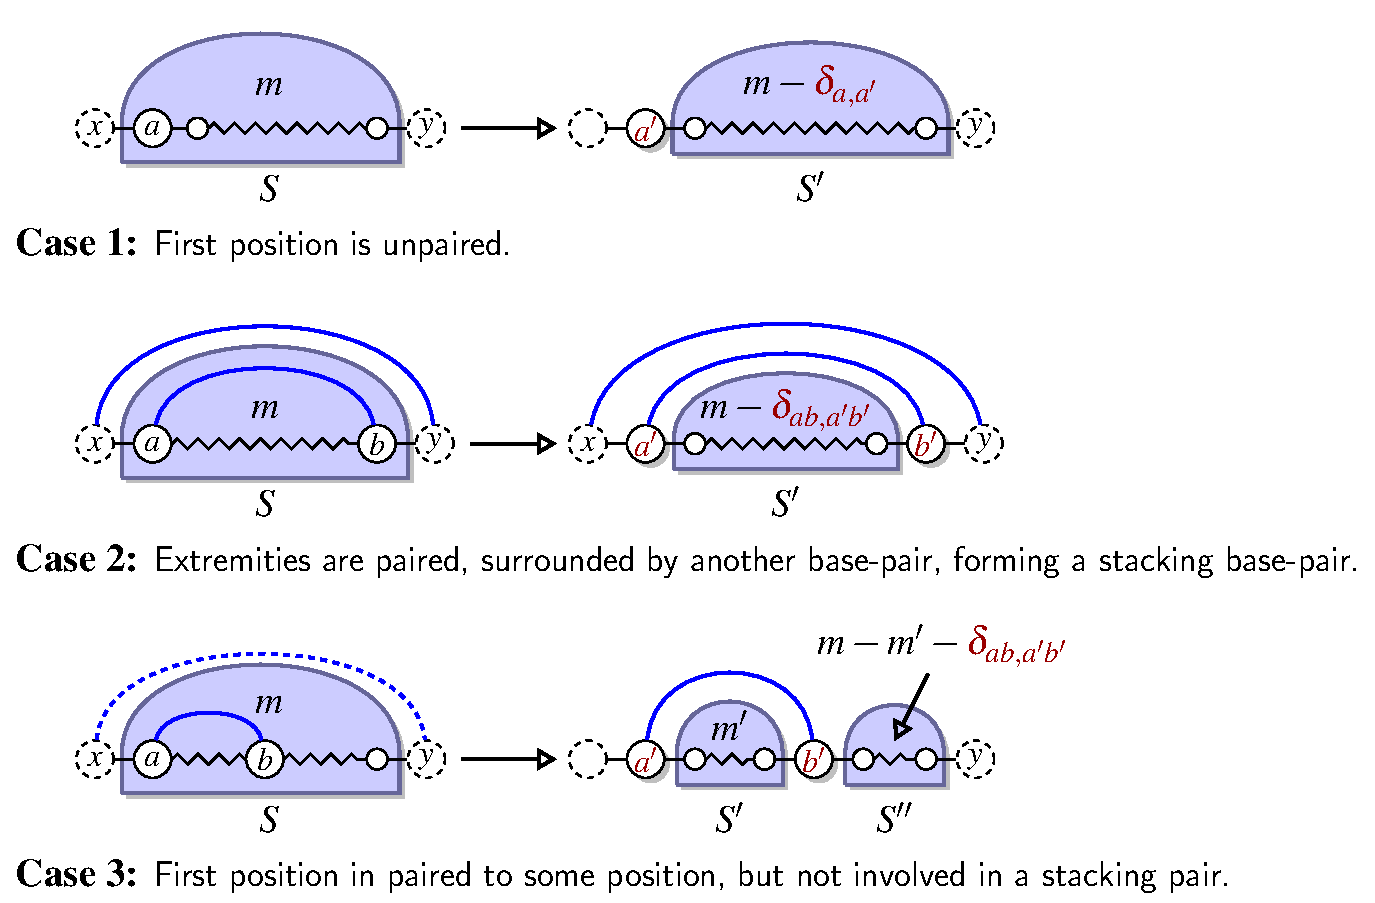
\includegraphics[scale=\ScaleDP]{FigDPInsideWrapper}
\caption{Principle of the inside computation (partition function). Any sequence (mutated)  
can be decomposed as a sequence preceded by a, possibly mutated, base 
(Unpaired case), a sequence surrounded by some base-pair (Stacking-pair case), 
or as two sequences segregated by some base-pair (General base-pairing case). In this latter case, mutations must be distributed between sub-sequences.\label{fig:inside}}
\end{figure}

The \emph{Inside} function $\Z{\Struct}{m}{x,y}$ is simply the partition function, i.e. the sum of Boltzmann factors over all sequences for a substructure $\Struct$ (implicitly attached to an interval $[i,j]$ of the sequence), featuring $m$ mutations/errors compared to $s$, and having flanking nucleotides $x$ and $y$. 
Such terms can be computed recursively, using the following equation for the initial case:
\begin{equation}
	\forall x,y\in \B\times \B, m\in [0,M]:\, \Z{\varepsilon}{m}{x,y}=\left\{
	\begin{array}{ll}
		1 &\text{ If } m = 0\\
		0 &\text{ Otherwise.}
	\end{array}\right.
\label{eq:Z_in}
\end{equation}
In other words, either there is no sequence at distance $m>0$ of the empty sequence, or the only allowed sequence is the empty sequence ($m=0$), having energy $0$. Since the contributions only depend on base pairs, they do not appear in the initial conditions. 

The main recursion considers a general structure $\Struct$, flanked by two nucleotides (outside the region of interest) $x$ and $y$, respectively on the $5'$ and $3'$ end of the sequence. As illustrated by Figure~\ref{fig:inside}, it is computed, for each subinterval $[i,j]$, by considering one of the three following cases, dependent on the base-pairing status and context of the leftmost position in the sequence/structure:
\begin{itemize}
\item {\bf Case 1: Unpaired leftmost position.} If the first position  is unpaired in the structure, then $\Struct$ can be further decomposed, using a dot-parenthesis notation, as $\Struct = \ub \Struct'$. Let $a\in B$ be the nucleotide found at the leftmost position in the initial structure, then one has:
\begin{equation}
\label{eq:Z_rec_A}
	\Z{\Struct}{m}{x,y} =
      \sum_{\substack{a'\in \B,\\ \Kron_{a,a'}\le m}}  
      \Z{\Struct'}{m-\Kron_{a,a'}}{a',y}.
\end{equation}
Indeed, any suitable sequence is a concatenation of a, possibly mutated, nucleotide $a'$ at the first position, followed by a sequence over the remaining interval, having $m-\Kron_{a,a'}$ mutations (accounting for a possible mutation at first position), and having flanking nucleotides $a'$ and $y$.
\item {\bf Case 2: Paired ends, stacking onto another base-pair.} If both ends of the considered interval form a base-pair ($\Struct = \op\Struct'\cp$), stacking onto another base pair just outside whole region, then the isosteric contribution of the base-pair must be supplemented with a specific "stacking-pairs" bonus. Let $a$ and $b$ be the nucleotides found on both ends of the interval (positions $i$ and $j$), then one has
\begin{equation}
\label{eq:Z_rec_B}
	\Z{\Struct}{m}{x,y} =
      \sum_{\substack{a',b'\in \B^2,\\ \Kron_{ab,a'b'}\le m}}
			 e^{\frac{-\EBP{i,j}{xy}{a'b'}}{RT}}
			 \cdot \Z{S'}{m-\Kron_{ab,a'b'}}{a',b'}.
\end{equation}
Any sequence generated here consists of two, possibly mutated, nucleotides $a'$ and $b'$, flanking a sequence over the remaining portion. In order for the total distance to sum to $m$, this portion must feature $m-\Kron_{ab,a'b'}$ additional point wise mutations.

\item {\bf Case 3: Paired leftmost position, but no stacking pairs.} In this case, the structure is split into two parts by the base pair ($\Struct = \op \Struct'\cp\Struct''$). Let us denote by $k$ the partner of position $i$, and by $a$, $b$ and $c$ the bases found at positions $i$, $k$ and $j$ respectively, then one has:
\begin{equation}
\label{eq:Z_rec_C}
	\Z{\Struct}{m}{x,y}=\sum_{\substack{a',b'\in \B^2,\\ \Kron_{ab, a'b'}\le m}}
      \sum_{m'=0}^{m-\Kron_{ab,a'b'}}
   		 e^{\frac{-\EBP{i,k}{\varnothing}{a'b'}}{RT}}
      \cdot\Z{\Struct'}{m-m'-\Kron_{ab,a'b'}}{a',b'}
      \cdot\Z{\Struct''}{m'}{b',y}.
\end{equation}
In other words, if the leftmost position is paired, and the base-pair is not stacking onto another base-pair, then the  only term contributing directly to the energy is the isostericity of the base pair. Admissible sequences for $\Struct$ consist of two paired nucleotides $a'$ and $b'$ at positions $i$ and $k$ respectively, flanking a sequence for $\Struct'$ (over an interval $[i+1,k-1]$), and followed by a (possibly empty) sequence for $\Struct''$ (over $[k+1,j]$). Since the total number of mutations sums to $m$, a parameter $m'$ is introduced to distribute the remaining mutations between the two sequences.
\end{itemize}



\subsubsection{Outside computation.}	

The \emph{Outside} function, $\Y{\Struct}{m}{x,y}$ is the partition function considering only the 
contributions of subsequences excluding a given structure/interval $\Struct$, occupying the open interval $]i,j[$ in the sequence, at Hamming distance exactly $m$ to the initial sequence $s$, and assuming that nucleotides $x$ and $y$ were previously chosen for $i+1$ and $j-1$, the outermost portions of the excluded structure.
The associated terms $\Y{\Struct}{m}{x,y}$ can then be computed recursively, initially considering the case of any prefix $\Struct'$ of the complete structure:
\begin{equation}
	\forall x,y\in \B\times \B, \forall \Struct'\text{ s.t. }\Struct=\Struct'.\Struct'', m\in [0,M]:\, \Y{\Struct'}{m}{x,y}=\Z{\Struct''}{m}{y,z}
\label{eq:Y_in}
\end{equation}
where $z\in\B$ can be any nucleotide, and provably does not affect further computations. 
In other words, the sequences explored by an outside computation, excluding a prefix of $\Struct$, are exactly the sequences generated on the corresponded suffix. This set of sequence is also the inside term on the suffix structure.
It is also worth pointing out that $\Y{\Struct}{m}{x,y}= \Z{\varepsilon}{m}{y,X}=\mathbbm{1}_{m=0}$.

\begin{figure}[t]\centering
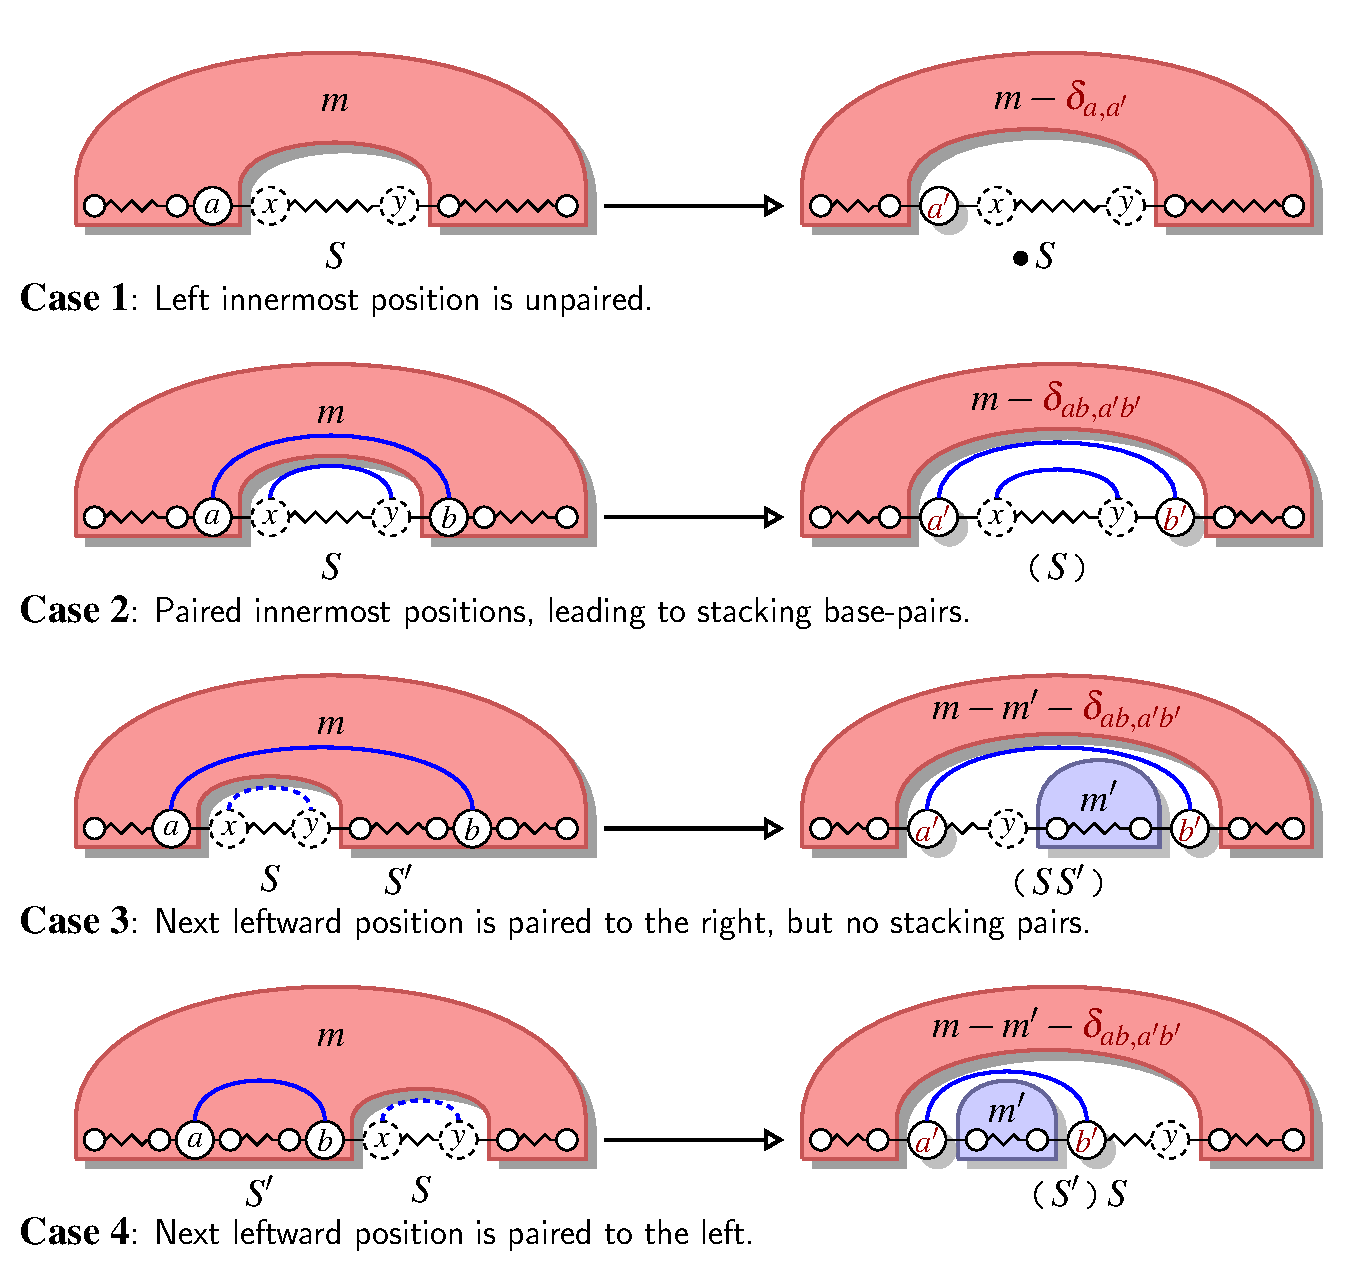
\includegraphics[scale=\ScaleDP]{FigDPOutsideWrapper}
\caption{Principle of the outside computation. Note that the outside algorithm uses intermediate results from the inside algorithm, 
therefore its efficient implementation requires the precomputation and storage of the inside contributions.\label{fig:outside}}
\end{figure}
In general, the main recurrence below works by extending the excluded structure $\Struct$ (covering the $]i,j[$ interval) in the leftward direction. As shown in Figure~\ref{fig:outside}, four cases must be considered, depending on the base-pairing status and directionality of the next considered position:
\begin{itemize}
\item {\bf Case 1: Unpaired position.} When the innermost leftward base is unpaired, any base $a\in\B$ may be chosen for this position, and the rest of the sequence is generated recursively. The number of remaining mutations may be decreased by the choice of $a$, leading to the following recurrence:
\begin{equation}
	\Y{\Struct}{m}{x,y} = \sum_{\substack{a'\in \B,\\ \Kron_{a,a'}\le m}}
    \Y{\ub\Struct}{m- \Kron_{a,a'}}{a',y}
\label{eq:Y_rec_A}
\end{equation}
\item {\bf Case 2: Stacking base-pair.} If both ends of the excluded structure are paired together, and are nested within another base-pair in the remaining structure, then an additional contribution, stemming from a stacking pairs energy, has to be considered. The outside terms are then computed by simulating any pair of base-pairing nucleotides for $i,j$, and by proceeding recursively on the remaining portion, as follows:
\begin{equation}
	\Y{\Struct}{m}{x,y} = 
    \sum_{\substack{a'b'\in \B^2,\\ \Kron_{ab,a'b'}\le m}}
		 e^{\frac{-\EBP{i,j}{xy}{a'b'}}{RT}}\cdot
    \Y{\op\Struct\cp}{m- \Kron_{ab,a'b'}}{a',b'} 
\label{eq:Y_rec_B}
\end{equation}
\item {\bf Case 3: Next position paired rightward, in the absence of stacking pair.} In this case, the innermost leftward position $i$ is paired to the right at some position $k$ . 
Let us assume that its partner resides outside the excluded structure $\Struct$ (This assumption is provably without loss of generality, and directly follows from the fact that $\Struct$ is well-parenthesized). 
The structure within the base-pair may be described by the expression $\op\Struct \Struct'\cp$, where $\Struct'$ may possibly be empty (except if $\Struct$ is enclosed within corresponding brackets, to avoid stacking pairs). Therefore, any sequence considered by the outside computation consists in three independent parts: two nucleotides for the paired positions, a sequence for the region excluding $\Struct''$, and a sequence for $\Struct'$. It follows that:
\begin{equation}
	\Y{\Struct}{m}{x,y} = \sum_{\substack{a'b'\in \B^2,\\ \Kron_{ab,a'b'}\le m}}
		 \sum_{m'=0}^{m-\Kron_{ab,a'b'}}
  		 e^{\frac{-\EBP{i,k}{\varnothing}{a'b'}}{RT}}
		 \cdot\Y{\op\Struct \Struct'\cp}{m- \Kron_{ab,a'b'} - m'}{a',b'}
     \cdot\Z{\Struct'}{m'}{y,b'} .
\label{eq:Y_rec_C}
\end{equation}
\item {\bf Case 4: Next position paired leftward.} If the innermost, leftward, position $i$ is paired to some position $k<i$, delimiting a substructure $\Struct'$, then any sequence considered by the outside computation consists in three parts: two nucleotides $a$ and $b$, a sequence for $\Struct'$, and a sequence for the region excluding $\op\Struct'\cp\Struct$. Consequently, one has:
\begin{equation}
	\Y{\Struct}{m}{x,y} = 
		 \sum_{\substack{a'b'\in \B^2,\\ \Kron_{ab,a'b'}\le m}}
		 \sum_{m'=0}^{m-\Kron_{ab,a'b'}}
   	 e^{\frac{-\EBP{k,i}{\varnothing}{a'b'}}{RT}}
		 \cdot\Y{\op\Struct'\cp\Struct}{m- \Kron_{ab,a'b'} - m'}{a',b}
     \cdot\Z{\Struct'}{m'}{a',b'}
\label{eq:Y_rec_D}
\end{equation}
\end{itemize}

\subsubsection{Combining Inside and Outside Computations into Point-Wise Mutations Probabilities.}


We are now left to compute the probability that a a given nucleotide $a\in\B$ is found at a given position $i$.
This quantity can also be expressed as the ratio of $\mathcal{W}^M_{\substack{i, [a]}}$, the total Boltzmann weight 
of the set of sequences featuring the nucleotide, and $\Z{\varepsilon}{\le M}{X,X}$ the total weight of sequences having at most $M$ mutations:
\begin{equation}
	\mathbb{P}(s_i = a\;|\; M) := \frac{\mathcal{W}^M_{\substack{i, [a]}}}{\Z{\varepsilon}{\le M}{X,X'}} = \frac{\mathcal{W}^M_{\substack{i, [a]}}}{\sum_{m=0}^{M}\Z{\varepsilon}{m}{X,X'}}\label{eq:normalize}
\end{equation}
where $X,X'\in\B$ may be any nucleotides (no impact on energy/weights).

\begin{figure}[t]\centering
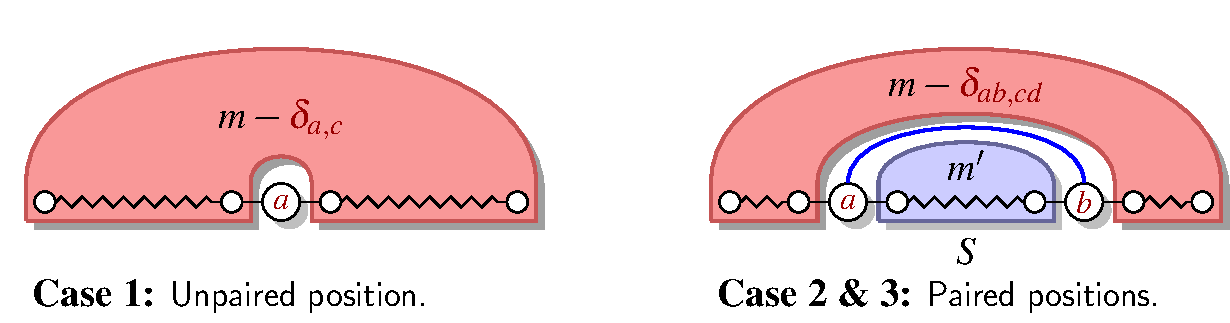
\includegraphics[scale=\ScaleDP]{FigDPCombineWrapper}
\caption{Combining the inside and outside contributions to compute the total Boltzmann weight of all sequences having a given base (case 1) or base-pair (cases 2 and 3) at a given position.\label{fig:combine}}
\end{figure}

To that purpose, one leverages the \emph{Inside-Outside} construction, as  illustrated by Figure~\ref{fig:combine}. Namely, while computing the total contribution of sequences featuring a base $a'\in\B$ at position $i$, one must consider the three following situations:
\begin{itemize}
\item {\bf Case 1: Unpaired position.} In this case, the supporting sequences are simply those excluding the structure $\ub$ at position $i$, where a base $c\in\B$ was formerly found. Summing over any possible number of mutations for the \emph{outside} region, one obtains:
\begin{equation}
 \mathcal{W}^M_{\substack{i, [a]}} =  \sum_{m=\Kron_{a,c}}^{M}
			\Y{\ub}{m-\Kron_{a,c}}{a,a}.
\label{eq:combine_A}
\end{equation}
\item {\bf Case 2: Position is paired rightward.} Here, position $i$ is paired to some position $k>i$, whose content impacts the base-pair contribution. Any sequence having $a$ at position $i$ can be decomposed as a base-pair, nesting a sequence for the structure $\Struct'$ on the interval $[i+1,k-1]$, and an outside sequence, excluding the structure $\op\Struct'\cp$.
Consequently, let $c$ and $d$ be the original nucleotides at positions $i$ and $k$, one has:
\begin{equation}
 \mathcal{W}^M_{\substack{i, [a]}} =  
			\sum_{m=0}^{M}
			\sum_{\substack{b\in \B\\\Kron_{ab,cd}\leq m}}
			\sum_{m'=0}^{m-\Kron_{ab,cd}}
     	 e^{\frac{-\EBP{i,k}{\varnothing}{ab}}{RT}}
			\cdot\Y{\op\Struct'\cp}{m-\Kron_{ab,cd}}{a,b}
			\cdot\Z{\Struct'}{m'}{a,b}
\label{eq:combine_B}
\end{equation}
\item {\bf Case 3: Position is paired leftward.} This case is symmetrical to the previous one, with the exception that $k<i$.
Consequently, let $c$ and $d$ be the original nucleotides at positions $i$ and $k$, one has:
\begin{equation}
 \mathcal{W}^M_{\substack{i, [a]}} =  
			\sum_{m=0}^{M}
			\sum_{\substack{b\in \B\\\Kron_{ba,cd}\leq m}}
			\sum_{m'=0}^{m-\Kron_{ba,cd}}
     	 e^{\frac{-\EBP{k,i}{\varnothing}{ba}}{RT}}
			\cdot\Y{\op\Struct'\cp}{m-\Kron_{ba,cd}}{b,a}
			\cdot\Z{\Struct'}{m'}{b,a}
\label{eq:combine_C}
\end{equation}
\end{itemize}

\subsection{Complexity Considerations}
Using dynamic programming, Equations~\eqref{eq:Z_rec_A}-\eqref{eq:Z_rec_C} and~\eqref{eq:Y_rec_A}-\eqref{eq:Y_rec_D} can be computed in linear time and memory. Namely, the $\mathcal{Z}^{*}_{*}$ and $\mathcal{Y}^{*}_{*}$ terms are computed starting from smaller values of $m$ and structure lengths, storing the results as they become available to ensure constant-time access during later stages of the computation. Furthermore, energy terms $E(\cdot)$ may be accessed in constant time after a simple precomputation of the isostericity contributions in $\Theta(n\cdot|\Omega|)$. Computing any given term therefore requires $\Theta(m)$ operations due to the explicit distribution of the number of mutations.

In principle, $\Theta(M\cdot n^2)$ terms, identified by different $(\Struct,m)$ triplets, should be computed.
However, a close inspection of the recurrences reveals that the computation can be safely restricted to a subset of intervals $(i,j)$.
For instance, the inside algorithm only requires computing intervals $[i,j]$ that do not break any base-pair, and whose next position $j+1$ is either past the end of the sequence, or is base-paired prior to $i$. A similar property holds for the outside computation,  following from the linearity of the outside recurrence (i.e. the computation of the outside term for a given excluded structure only relies on the computation of another, strictly larger, structure).
 
These properties drastically limit the combinatorics of required computations, dropping from $\Theta(n^2)$ to $\Theta(n)$ the number of terms that need to be computed and stored. Consequently the overall complexity of the algorithm is $\Theta(n\cdot(|\Omega|+M^2))$ arithmetic operations and $\Theta(n\cdot(|\Omega|+M))$ memory.
